\documentclass[11pt,a4paper]{article}
\usepackage[utf8]{inputenc}
\usepackage[spanish]{babel}	%Idioma
\usepackage{amsmath}
\usepackage{amsfonts}
\usepackage{amssymb}
\usepackage{graphicx} 	%Añadir imágenes
\usepackage{geometry}	%Ajustar márgenes
\usepackage[export]{adjustbox}[2011/08/13]
\usepackage{float}
\restylefloat{table}
\usepackage[hidelinks]{hyperref}
\usepackage{titling}
\graphicspath{{/home/nazaret/Escritorio/LaTEX}}
%\usepackage{minted}
\usepackage{multirow}
\usepackage{caption}
\usepackage{multicol}
\usepackage[shortlabels]{enumitem}
\usepackage{array}
\selectlanguage{spanish}

%Opciones de encabezado y pie de página:
\usepackage{fancyhdr}
\pagestyle{fancy}
\lhead{Nazaret Román Guerrero}
\rhead{Redes Multiservicio}
\lfoot{Grado en Ingeniería Informática}
\cfoot{}
\rfoot{\thepage}
\renewcommand{\headrulewidth}{0.4pt}
\renewcommand{\footrulewidth}{0.4pt}

%Opciones de fuente:
\usepackage[utf8]{inputenc}
\usepackage[default]{sourcesanspro}
\usepackage{sourcecodepro}
\usepackage[T1]{fontenc}

\setlength{\parindent}{15pt}
\setlength{\headheight}{15pt}
\setlength{\voffset}{10mm}

% Custom colors
\usepackage{color}
\definecolor{deepblue}{rgb}{0,0,0.5}
\definecolor{deepred}{rgb}{0.6,0,0}
\definecolor{deepgreen}{rgb}{0,0.5,0}

\usepackage{listings}
\lstset{basicstyle=\ttfamily,
  showstringspaces=false,
  commentstyle=\color{red},
  keywordstyle=\color{blue}
}

\begin{document}
\begin{titlepage}

\begin{minipage}{\textwidth}

\centering
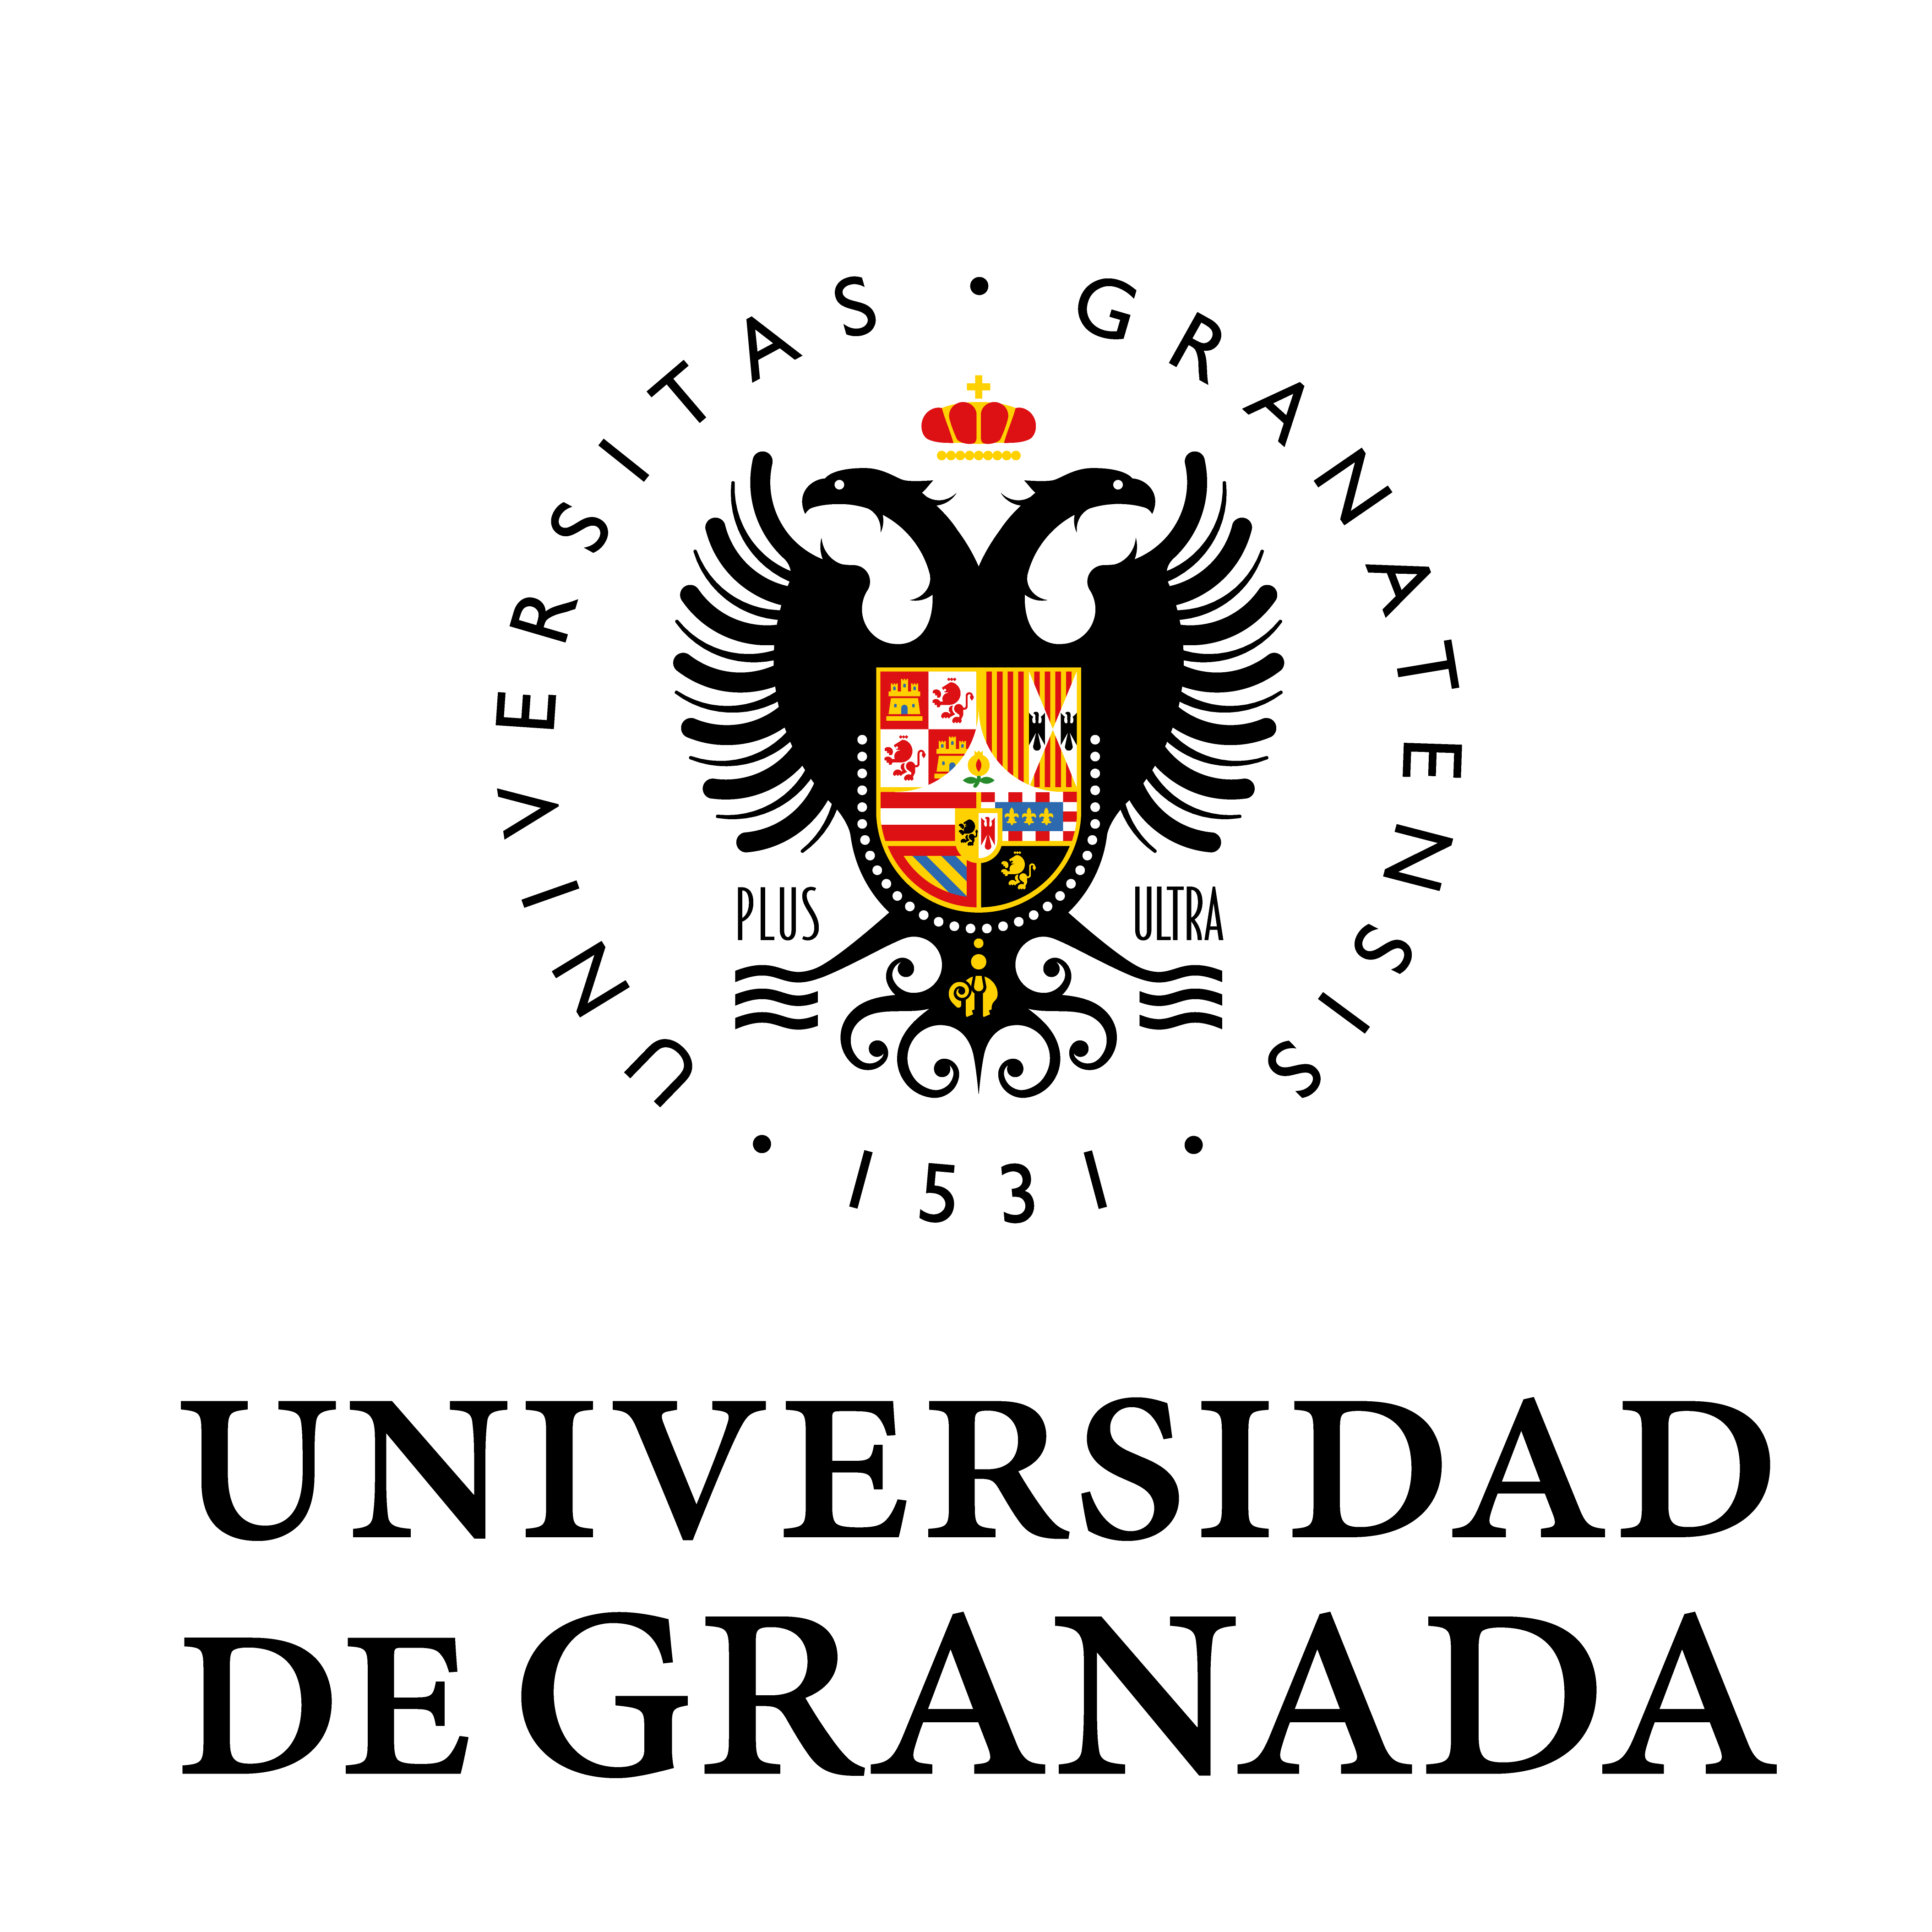
\includegraphics[width=0.5\textwidth]{img/logo.png}\\

\textsc{\Large asignatura\\[0.2cm]}
\textsc{GRADO EN INGENIERÍA INFORMÁTICA}\\[1cm]

{\Huge\bfseries Práctica 1\\}
\noindent\rule[-1ex]{\textwidth}{3pt}\\[3.5ex]
{\large\bfseries Configuración de un \textit{router} para la provisión de QoS según SLA}
\end{minipage}

\vspace{1.5cm}
\begin{minipage}{\textwidth}
\centering

\textbf{Autora}\\ {Nazaret Román Guerrero}\\[2.5ex]

\includegraphics[width=0.3\textwidth]{img/etsiit.jpeg}\\[0.1cm]
\vspace{1cm}
\textsc{Escuela Técnica Superior de Ingenierías Informática y de Telecomunicación}\\
\vspace{1cm}
\textsc{Curso 2018-2019}
\end{minipage}
\end{titlepage}

\pagenumbering{gobble}
\pagenumbering{arabic}
\tableofcontents
\thispagestyle{empty}

\newpage

\section{Configuración de los routers}

Para configurar el \textit{router} RA vamos a utilizar \textit{packettracer}. Elegimos un router, el modelo 1841 y comenzamos a configurarlo como en el laboratorio.\\

Primero entramos al modo de configuración y cambiamos el nombre del router mediante el comando\\

\begin{lstlisting}[language=bash,caption={Cambio de hostname},captionpos=b]
Router# hostname RA
\end{lstlisting}

Tras hacer esto configuramos las interfaces de red.\\

\begin{lstlisting}[language=bash,caption={Configuración de la interfaz FastEthernet 0/0},captionpos=b]
RA# interface FastEthernet 0/0
RA# ip address 10.1.1.100 255.255.255.0
RA# no shutdown
\end{lstlisting}

El último comando es necesario para levantar la interfaz. Hacemos lo mismo con la interfaz \texttt{FastEthernet 0/1}. El procedimiento completo se muestra en la imagen:

\begin{figure}[H]
	\centering
	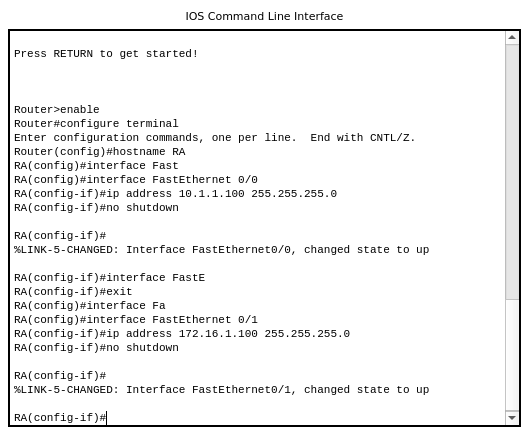
\includegraphics[scale=0.7]{img/RA-config.png}
\end{figure}

Para comprobar que todo está funcionando podemos utilizar el comando\\

\begin{lstlisting}[language=bash]
RA# show running-config
\end{lstlisting}

que muestra la siguiente salida:

\begin{figure}[H]
	\centering
	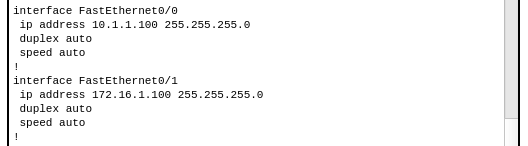
\includegraphics[scale=0.7]{img/show_running-config.png}
\end{figure}

También podemos situarnos encima del \textit{router}, donde aparece una burbuja de texto con las interfaces disponibles y su estado:

\begin{figure}[H]
	\centering
	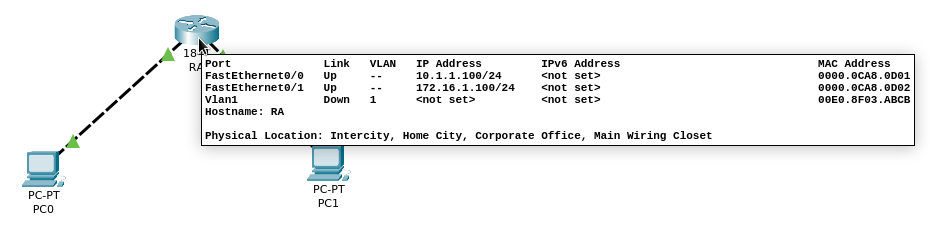
\includegraphics[scale=0.4]{img/bubble.png}
\end{figure}

\begin{figure}[H]
	\centering
	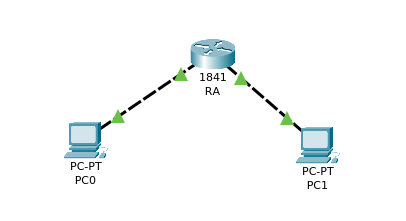
\includegraphics[scale=0.5]{img/topologia.png}
\end{figure}

Con esto hemos comprobado que la configuración es correcta, puesto que, además y como comprobación extra, el tráfico entre el \textit{router} y los PCs está viajando correctamente (indicado con las flechas verdes).

\newpage

\section{Tráfico con ITG y análisis con wireshark}

Para llevar a cabo este análisis, he creado una máquina virtual con Ubuntu 18.04 LTS donde he instalado ITG, tal y como se ve en la imagen:

\begin{figure}[H]
	\centering
	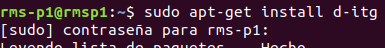
\includegraphics[scale=1.0]{img/d-itg-install.png}
\end{figure}

También he instalado wireshark para analizar el tráfico y poder calcucular las transferencias.

\subsection{¿Qué tasa de transferencia media y máxima requiere la aplicación \textit{Quake3}?}

Vamos a empezar con el tráfico de \textit{Quake3}. Para ello, vamos a generar el tráfico en localhost y también lo va a recibir localhost. Primero debemos empezar a capturar el tráfico con wireshark. Tras esto, en dos terminales diferentes lanzamos\\

\begin{lstlisting}[language=bash,caption={Recibir el tráfico},captionpos=b]
$ ITGRecv
\end{lstlisting}

\begin{lstlisting}[language=bash,caption={General el tráfico},captionpos=b]
$ ITGSend -a locahost -rp 4444 -t 2000 -l quake3.log Quake3
\end{lstlisting}

para recibir el tráfico y generarlo respectivamente. Debemos hacerlo en ese orden. El tráfico se genera para ser enviado a localhost, a través del puerto 4444 durante 2000 milisegundos (2 segundos). Toda la información se guarda en el archivo de logs quake3.log.\\

Una vez finalizada la generación de tráfico, guardamos la captura de wireshark, donde vamos a sacar los datos necesarios.\\

Para extraer estos datos necesitamos hacer cálculos. Utilizando el archivo \texttt{.csv} que hemos guardado del tráfico capturado por wireshark los vamos a calcular. Un fragmento con los primeros paquetes enviados es el siguiente:

\begin{table}[H]
\centering
\begin{tabular}{|c|c|c|c|c|c|c|}
\hline
  & \textbf{Time}        & \textbf{Source}    & \textbf{Destination} & \textbf{Protocol} & \textbf{Length} & \textbf{Packet bytes} \\ \hline
1  & 0.007007187 & 127.0.0.1 & 127.0.0.1   & UDP      & 106    & 62           \\ \hline
2  & 0.014563362 & 127.0.0.1 & 127.0.0.1   & UDP      & 114    & 70           \\ \hline
3  & 0.025882455 & 127.0.0.1 & 127.0.0.1   & UDP      & 108    & 64           \\ \hline
4  & 0.038729095 & 127.0.0.1 & 127.0.0.1   & UDP      & 104    & 60           \\ \hline
5  & 0.044081841 & 127.0.0.1 & 127.0.0.1   & UDP      & 112    & 68           \\ \hline
6  & 0.059141921 & 127.0.0.1 & 127.0.0.1   & UDP      & 103    & 59           \\ \hline
7  & 0.064262957 & 127.0.0.1 & 127.0.0.1   & UDP      & 103    & 59           \\ \hline
8  & 0.072172963 & 127.0.0.1 & 127.0.0.1   & UDP      & 112    & 68           \\ \hline
9 & 0.084276246 & 127.0.0.1 & 127.0.0.1   & UDP      & 107    & 63           \\ \hline
10 & 0.086532722 & 127.0.0.1 & 127.0.0.1   & UDP      & 106    & 62           \\ \hline
11 & 0.086545362 & 127.0.0.1 & 127.0.0.1   & UDP      & 101    & 57           \\ \hline
12 & 0.087990486 & 127.0.0.1 & 127.0.0.1   & UDP      & 100    & 56           \\ \hline
13 & 0.088165962 & 127.0.0.1 & 127.0.0.1   & UDP      & 106    & 62           \\ \hline
14 & 0.094765568 & 127.0.0.1 & 127.0.0.1   & UDP      & 112    & 68           \\ \hline
15 & 0.105661899 & 127.0.0.1 & 127.0.0.1   & UDP      & 107    & 63           \\ \hline
16 & 0.111843240 & 127.0.0.1 & 127.0.0.1   & UDP      & 110    & 66           \\ \hline
17 & 0.114155722 & 127.0.0.1 & 127.0.0.1   & UDP      & 106    & 62           \\ \hline
18 & 0.118700821 & 127.0.0.1 & 127.0.0.1   & UDP      & 110    & 66           \\ \hline
19 & 0.123173911 & 127.0.0.1 & 127.0.0.1   & UDP      & 103    & 59           \\ \hline
\end{tabular}
\caption{Paquetes de \textit{Quake3}}
\end{table}

A pesar de que aquí solo he puesto unos pocos, se envían un total de 192 paquetes en 2 segundos. Haciendo la suma de los bytes enviados en cada paquete hay un total de 12174 bytes. Es fácil saber que se envían 6087 bytes por segundo.

\begin{itemize}
	\item \textbf{Transferencia máxima}: Calculando la diferencia entre el tiempo de dos envíos consecutivos podemos calcular qué paquete ha tenido una mayor tasa de transferencia. Para ello el número de bytes enviados entre el tiempo que ha tardado en enviarse. Así sabemos que el paquete con mayor tasa de transferencia ha sido el número 11, con una tasa de transferencia de 4905063 bytes por segundo (\textasciitilde 4 MB/s). Tarda solo 0.00001264 milisegundos en mandar 57 bytes.
	\item \textbf{Transferencia media}: Para calcular la transferencia media solo debemos calcular la división de todas las transferencias individuales entre el número de transferencias totales. Puesto que han sido 192 transferencias, el resultado es 54730.97 bytes por segundo (\textasciitilde 54 KB/s).
\end{itemize}

\subsection{¿Qué tasa de transferencia media y máxima requiere la aplicación \textit{VoIP}?}

Ahora vamos a calcular lo mismo pero para \textit{VoIP}.\\

Los comandos son similares, solo cambia el comando para generarlo ya que tendremos que indicar un nuevo archivo de log y también el tipo de tráfico a generar: tráfico de \textit{VoIP}.

\begin{lstlisting}[language=bash,caption={Recibir el tráfico},captionpos=b]
$ ITGRecv
\end{lstlisting}

\begin{lstlisting}[language=bash,caption={General el tráfico},captionpos=b]
$ ITGSend -a locahost -rp 4444 -t 2000 -l voip.log VoIP
\end{lstlisting}

Un fragmento de la captura de wireshark es el siguiente:

\begin{table}[H]
\centering
\begin{tabular}{|c|c|c|c|c|c|c|}
\hline
   & \textbf{Time} & \textbf{Source} & \textbf{Destination} & \textbf{Protocol} & \textbf{Length} & \textbf{Packet bytes} \\ \hline
1  & 0.007282496   & 127.0.0.1       & 127.0.0.1            & UDP               & 136             & 92                    \\ \hline
2  & 0.017672392   & 127.0.0.1       & 127.0.0.1            & UDP               & 136             & 92                    \\ \hline
3  & 0.028318222   & 127.0.0.1       & 127.0.0.1            & UDP               & 136             & 92                    \\ \hline
4  & 0.043188033   & 127.0.0.1       & 127.0.0.1            & UDP               & 136             & 92                    \\ \hline
5  & 0.053422244   & 127.0.0.1       & 127.0.0.1            & UDP               & 136             & 92                    \\ \hline
6  & 0.063744400   & 127.0.0.1       & 127.0.0.1            & UDP               & 136             & 92                    \\ \hline
7  & 0.075721966   & 127.0.0.1       & 127.0.0.1            & UDP               & 136             & 92                    \\ \hline
8  & 0.095680083   & 127.0.0.1       & 127.0.0.1            & UDP               & 136             & 92                    \\ \hline
9  & 0.106023316   & 127.0.0.1       & 127.0.0.1            & UDP               & 136             & 92                    \\ \hline
10 & 0.118233078   & 127.0.0.1       & 127.0.0.1            & UDP               & 136             & 92                    \\ \hline
11 & 0.135999410   & 127.0.0.1       & 127.0.0.1            & UDP               & 136             & 92                    \\ \hline
12 & 0.146091480   & 127.0.0.1       & 127.0.0.1            & UDP               & 136             & 92                    \\ \hline
13 & 0.158204295   & 127.0.0.1       & 127.0.0.1            & UDP               & 136             & 92                    \\ \hline
14 & 0.170198676   & 127.0.0.1       & 127.0.0.1            & UDP               & 136             & 92                    \\ \hline
15 & 0.185968223   & 127.0.0.1       & 127.0.0.1            & UDP               & 136             & 92                    \\ \hline
16 & 0.196202404   & 127.0.0.1       & 127.0.0.1            & UDP               & 136             & 92                    \\ \hline
17 & 0.208900369   & 127.0.0.1       & 127.0.0.1            & UDP               & 136             & 92                    \\ \hline
18 & 0.224401892   & 127.0.0.1       & 127.0.0.1            & UDP               & 136             & 92                    \\ \hline
19 & 0.235904677   & 127.0.0.1       & 127.0.0.1            & UDP               & 136             & 92                    \\ \hline
20 & 0.250503915   & 127.0.0.1       & 127.0.0.1            & UDP               & 136             & 92                    \\ \hline
\end{tabular}
\caption{Paquetes de VoIP}
\end{table}

En este caso los paquetes tardan algo más en ser enviados, así que hay menos en 2 segundos. Se envían 157 paquetes, en contraste con los 192 de \textit{Quake3}, pero también son más grandes, ya que todos tienen un tamaño de 92 bytes por paquete.

\begin{itemize}
	\item \textbf{Transferencia máxima}: Al igual que en el caso anterior, calculamos la diferencia entre envíos y buscamos la mayor. Corresponde con el último paquete enviado: se envían 18410 bytes por segundo (\textasciitilde 17 KB/s), concretamente en este caso se envían 92 bytes en 0.004997281 milisegundos.
	\item \textbf{Transferencia media}: Utilizando la división de las transferencias individuales entre el número de envíos sabemos que el resultado es 5539.32 bytes por segundo (\textasciitilde 5 KB/s).
\end{itemize}

\subsection{Gráficas y retardos entre paquetes}

Como es evidente, el tiempo de envío varía de un paquete a otro, por diversos motivos: congestion de la red, procesos presentes en el dispositivo que genera el tráfico o en el que lo recibe...\\

Para ver la diferencia entre el tiempo de envíos podemos usar una gráfica tomado algunos valores (todos los valores es inviable puesto que el gráfico se ve tan apretado que no se puede leer). En el eje X están representados los tamaños de los paquetes y en el eje Y el tiempo que han tardado en enviarse.

\begin{itemize}
	\item \textbf{\textit{Quake3}}. Se han tomado 21 valores, ya que se aprecia bien los saltos de tiempo entre un paquete y otro.
	\begin{figure}[H]
		\centering
		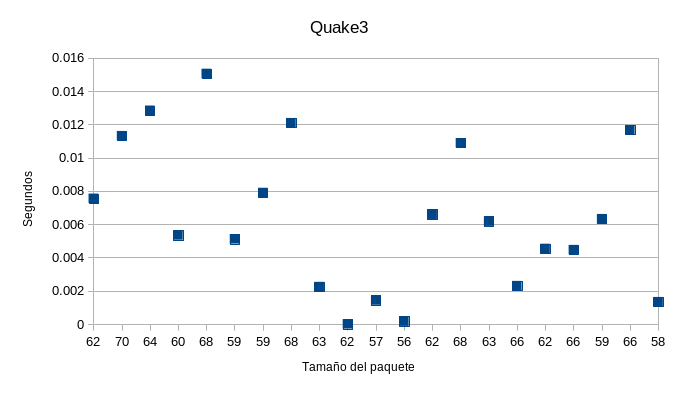
\includegraphics[scale=0.7]{img/quake3-grafica.png}
	\end{figure}
	
	\item \textbf{\textit{VoIP}}. En este caso se han cogido 30 valores, ya que las variaciones son menos evidentes que en el caso de \textit{Quake3}.
	\begin{figure}[H]
		\centering
		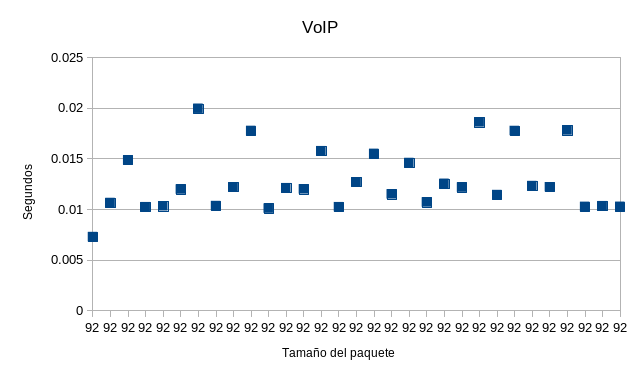
\includegraphics[scale=0.7]{img/voip-grafica.png}
	\end{figure}
\end{itemize}

\newpage

\section{\textit{Shaping}}

Antes de configurar el \textit{shaping}, es necesario crear una clase que sirva para tráfico de \textit{Quake3}, que será sobre el que aplicaremos la política.\\

Para ello, creamos la clase tal y como se ve en la imagen. Se crea una lista de acceso que permite el tráfico de UPD que vaya dirigido al puerto 6666, de cualquier fuente y a cualquier destino. Una vez hecha la lista, se crea la clase obligando a que el tráfico de dicha clase coincida con las reglas impuestas en la lista de acceso que hemos creado.

\begin{figure}[H]
	\centering
	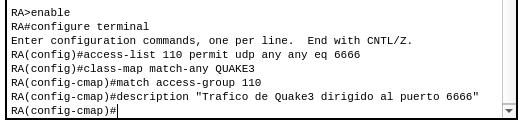
\includegraphics[scale=0.7]{img/class-map.png}
\end{figure}

Al ejecutar el comando \texttt{show running-config} aparece un fragmento como este (no se ha puesto la salida entera porque no cabía en una sola captura y solo interesaba esta parte):

\begin{figure}[H]
	\centering
	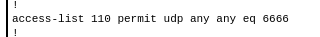
\includegraphics[scale=0.7]{img/show-running-config-access-list.png}
\end{figure}

Ahora vamos a configurar el \textit{shaping}. Para ello establecemos una política que permita 112 Kbps y se lo aplicamos a la clase que hemos creado para el tráfico de \textit{Quake3}. El procedimiento se puede ver en la siguiente imagen:

\begin{figure}[H]
	\centering
	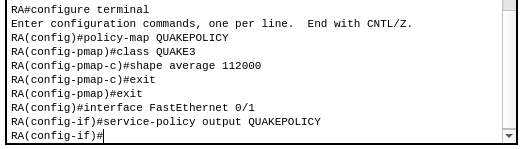
\includegraphics[scale=0.7]{img/shaping.png}
\end{figure}

Para comprobar que lo hemos hecho bien y que el \textit{shaping} ha sido aplicado, vamos a mostrar la configuración mediante el comando \texttt{show policy-map}:

\begin{figure}[H]
	\centering
	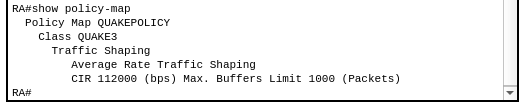
\includegraphics[scale=0.7]{img/show-shaping.png}
\end{figure}

Además vamos a mostrar la configuración que se está ejecutando en el \textit{router} actualmente mediante el comando \texttt{show running-config}, cuya salida es la siguiente:

\begin{figure}[H]
	\centering
	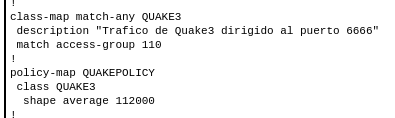
\includegraphics[scale=0.7]{img/show-running-config-shaping.png}
\end{figure}

Donde podemos ver que la clase y la política con \textit{shaping} están configuradas correctamente y son la configuración actual del \textit{router}. Puesto que el \textit{policy} no está disponible en los \texttt{routers}, no podemos hacer una comparativa con el \textit{shaping}.

\newpage

\section{QoS en el router RA}

Vamos a ofrecer QoS a través de nuestro router. Para ello, vamos a crear varias clases, una por cada tipo de tráfico que vamos a filtrar: una para \textit{VoIP}, otra para \textit{Quake3} y otra para el resto de tráfico.\\

Para ello, configuramos las clases, el \texttt{policy-map} y el \textit{shaper} de cada una tal y como se ve en las imágenes de abajo: primero el de \textit{VoIP}, después \textit{Quake3} y por último la clase por defecto. Tras esto, se añaden a la interfaz FastEthernet 0/0.

\begin{figure}[H]
	\centering
	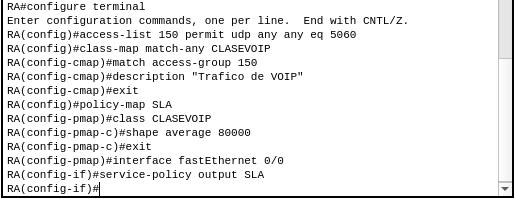
\includegraphics[scale=0.7]{img/voip-ej5.png}
\end{figure}

\begin{figure}[H]
	\centering
	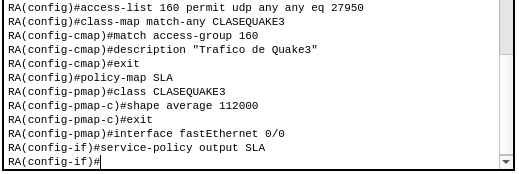
\includegraphics[scale=0.7]{img/quake-ej5.png}
\end{figure}

\begin{figure}[H]
	\centering
	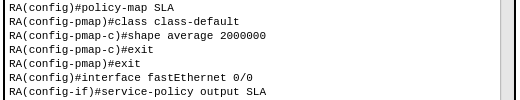
\includegraphics[scale=0.7]{img/class-default-ej5.png}
\end{figure}

Como se puede ver, a cada uno se le ha asignado un valor para los bps. Una vez creados, vamos a mostrar la configuración que se está ejecutando para saber que está funcionando correctamente. Al ejecutar \texttt{show running-config} podemos ver las clases de tráfico que tenemos:

\begin{figure}[H]
	\centering
	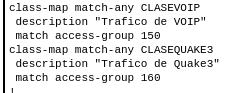
\includegraphics[scale=0.7]{img/classess-ej5.png}
\end{figure}

Vamos a comprobar que el \texttt{policy-map} está configurado correctamente y que está asignado a la interfaz FastEthernet 0/0. Como podemos ver en la imagen siguiente, el \texttt{policy-map} SLA consta de tres tráficos distintos, cada uno con un tasa de bits por segundo asignada.

\begin{figure}[H]
	\centering
	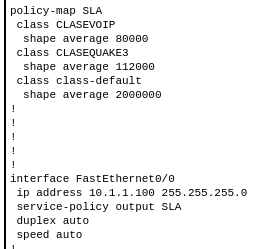
\includegraphics[scale=0.7]{img/policy-map-ej5.png}
\end{figure}

\end{document}